\documentclass{article}
\usepackage{graphicx}
\usepackage{geometry}
\geometry{margin=1.0in, top=1.0in, bottom=1.0in}
\usepackage{array}
\usepackage{multicol}
\usepackage{tikz}
\usepackage[skip=2pt,font=scriptsize]{caption}
\usepackage{subfig}
\graphicspath{{/Users/amandanewmark/repositories/galaxy_dark_matter/lumprofplots/clumps/}{/Users/amandanewmark/repositories/galaxy_dark_matter/lumprofplots/distribution/}}

 \title{Testing Photometry Issues in Luminous Red Galaxies}
 \author{Amanda Newmark}
 \date{August 2016}

\begin{document}
\begin{titlepage}
\maketitle
\end{titlepage}
\tableofcontents{}
\section{Introduction}

An objective of HSC Project is to understand the correlation between the star formation history and the mass assembly history of Luminous Red Galaxies (LRGs) through studying the slope of the luminosity density profiles.

In order to certify the validity of our results, it is essential that we test the photometric contamination caused by fainter galaxies that are not properly resolved, or \textit{deblended}. Such galaxies can saturate the apparent magnitude of the galaxy, most prominently at the outer stellar halo of the galaxy.

\begin{table}[h]
\centering
\begin{tabular}{||c||}
\hline
\textbf{Flags}  \\ 
\hline\hline
flags.pixel.interpolated.center  \\[1ex]
\hline
flags.pixel.edge \\
\hline
flags.pixel.saturated.center \\[1ex]
\hline
flags.pixel.cr.center \\
\hline
flags.pixel.bad \\
\hline 
flags.pixel.suspect.center \\[1ex]
\hline
flags.pixel.clipped any \\ [1ex]
\hline
\end{tabular}
\caption{Flag parameters in LOWZ}
\label{table:1}
\end{table}

The LOWZ catalogue flags specific galaxies we suspect have been contaminated. We determined that the LRGs flagged by at least one of the flags in Table \ref{table:1} influence the stacked luminosity profiles, and therefore it is necessary to disregard these galaxies. 

\section{Distinguishing Bright Center Objects}

\begin{figure}[h!]
\subfloat[Apparent Magnitude (m) Distribution\label{subfig:sfig11}]{ 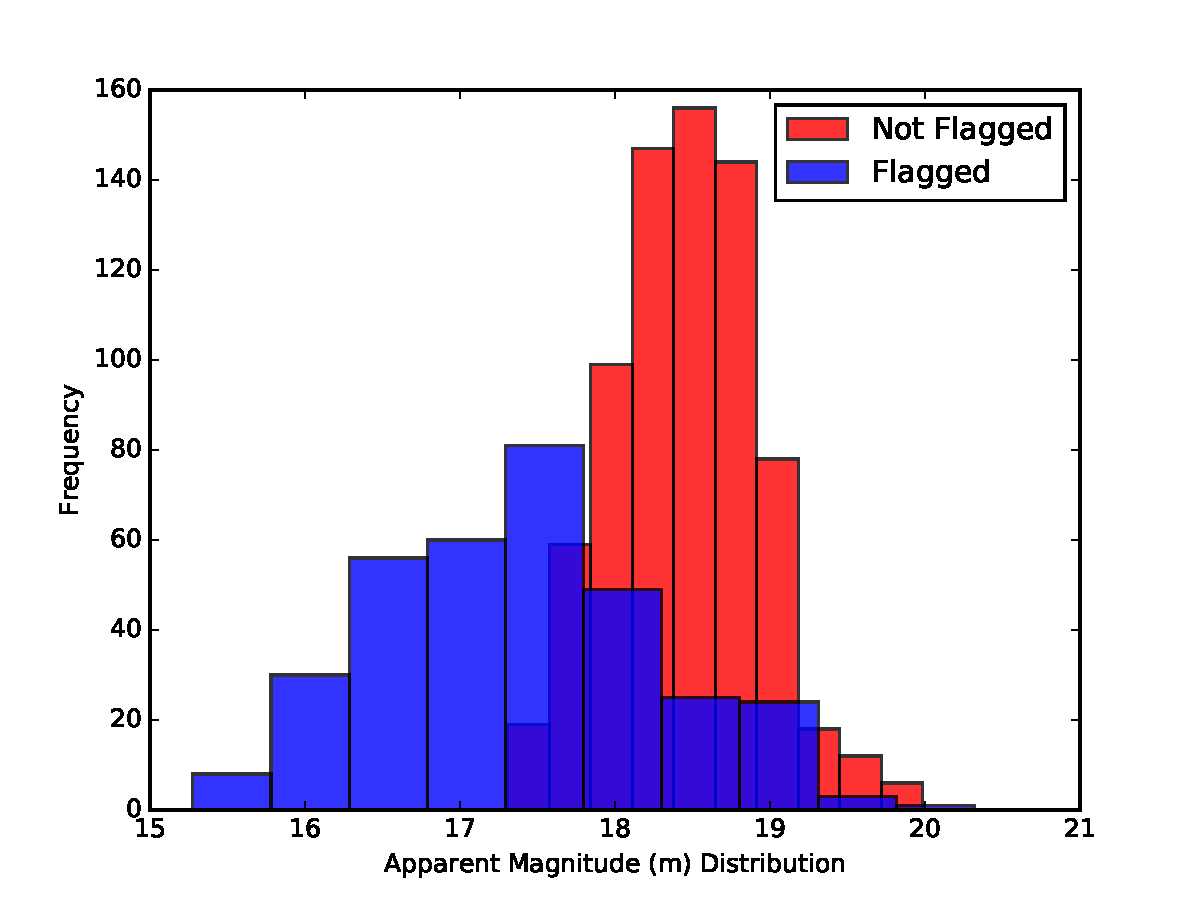
\includegraphics[width=0.5\textwidth]{3meanmagdist.pdf}}
\hfill
\subfloat[Redshift (Z) Distribution\label{subfig:sfig12}]{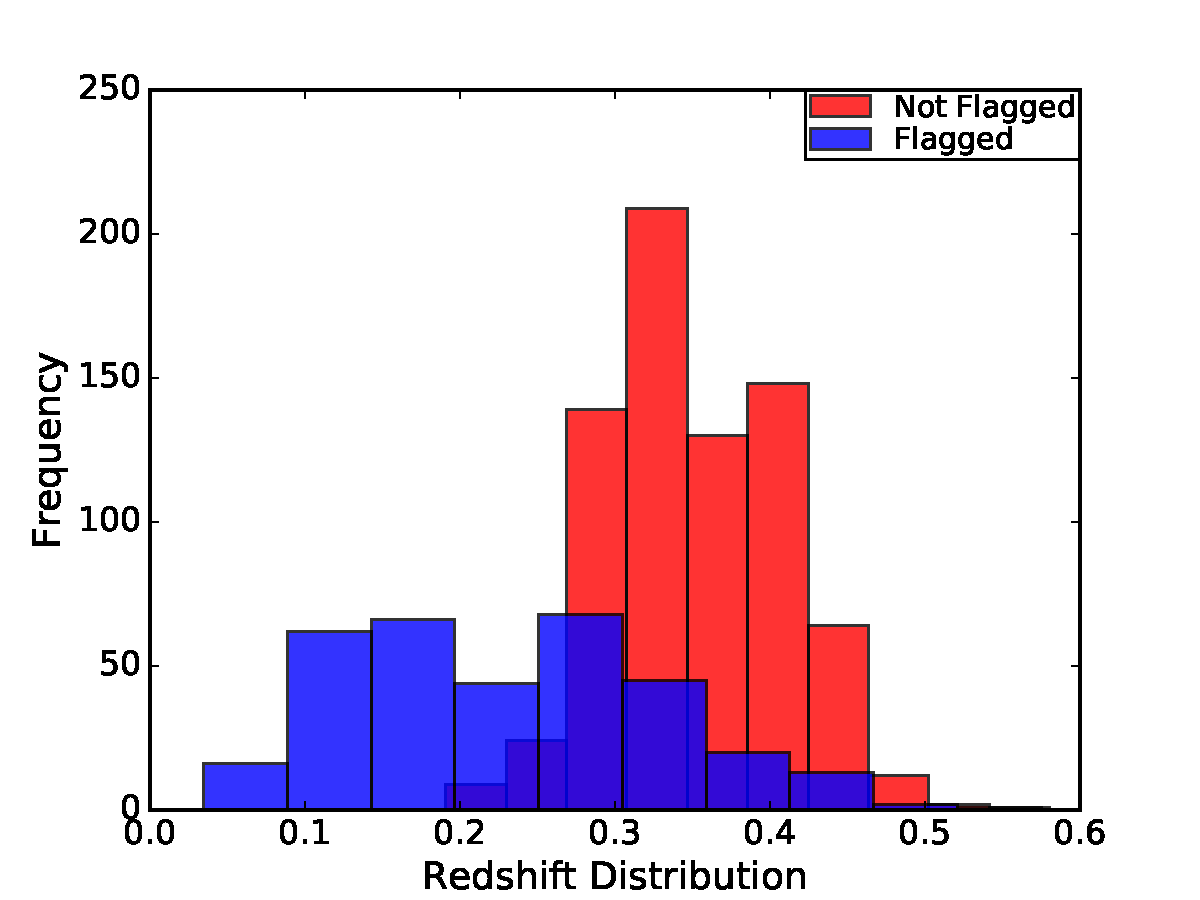
\includegraphics[width=0.5\textwidth]{3meanzdist.pdf}}
 \caption{With redshift cut: Stacked Luminosity Profile for LRG's flagged as Bright Center Objects (blue points), and those not flagged as Bright Center Objects (red points). }
\label{fig:mesha1}
\end{figure}

To determine whether bright object centers saturate our luminosity profiles, the LRGs are separated into two populations, one where flags.pixel.bright.object is \textbf{True} and one where flags.pixel.bright.object is \textbf{False}.  Since we first want to confirm that these galaxies are all from the same population, in Figure \ref{fig:mesha1}, we construct the distributions of the redshifts and apparent apparent magnitudes for flagged (blue bars) and not flagged (red bars) galaxies.

Varying parts of the stacked profile use distinct galaxies at different redshifts. As seen in Figure\ref{fig:mesha1}, the apparent magnitudes and redshifts for the flagged galaxies aren't normally distributed like the non-flagged galaxies. While the blue bars trail off at m=17, we also notice that they trail off at z=0.2. Since these galaxies were of lower redshift (as seen in Figure \ref{subfig:sfig12}), they appear to be more luminous (as seen in Figure \ref{subfig:sfig11}.) Since we are measuring intrinsic brightness, our stacked profile was falsely brighter.This is evidence that those LRGs are flagged as Bright Objects because they offset our stacked profile. Therefore, we set a lower limit of 0.2 to our redshift distribution.  

\begin{figure}[h!]
\subfloat[Luminosity Density Profiles\label{subfig:sfiga}]{ 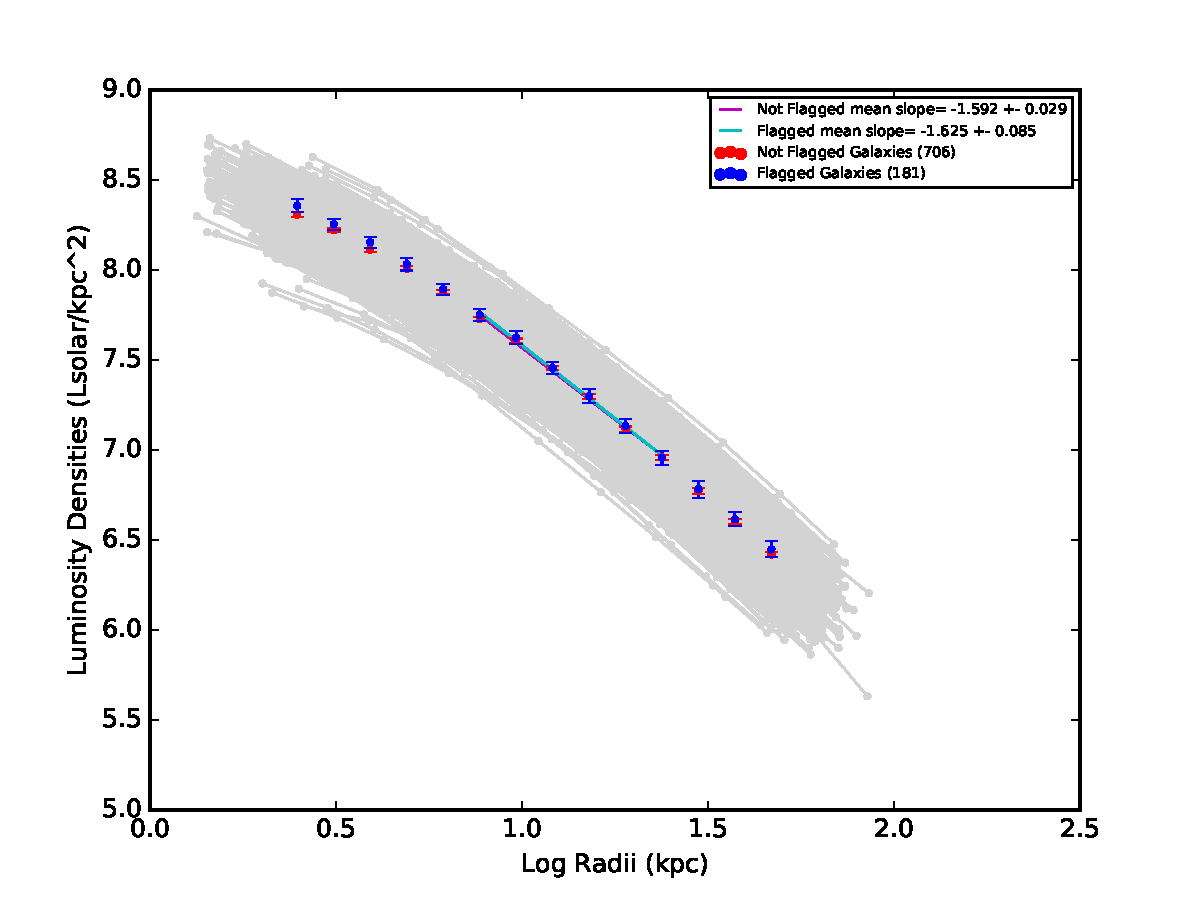
\includegraphics[width=0.5\textwidth]{3meanuplimTF.pdf}}
\hfill
\subfloat[Distribution of alpha\_star slopes\label{subfig:sfigb}]{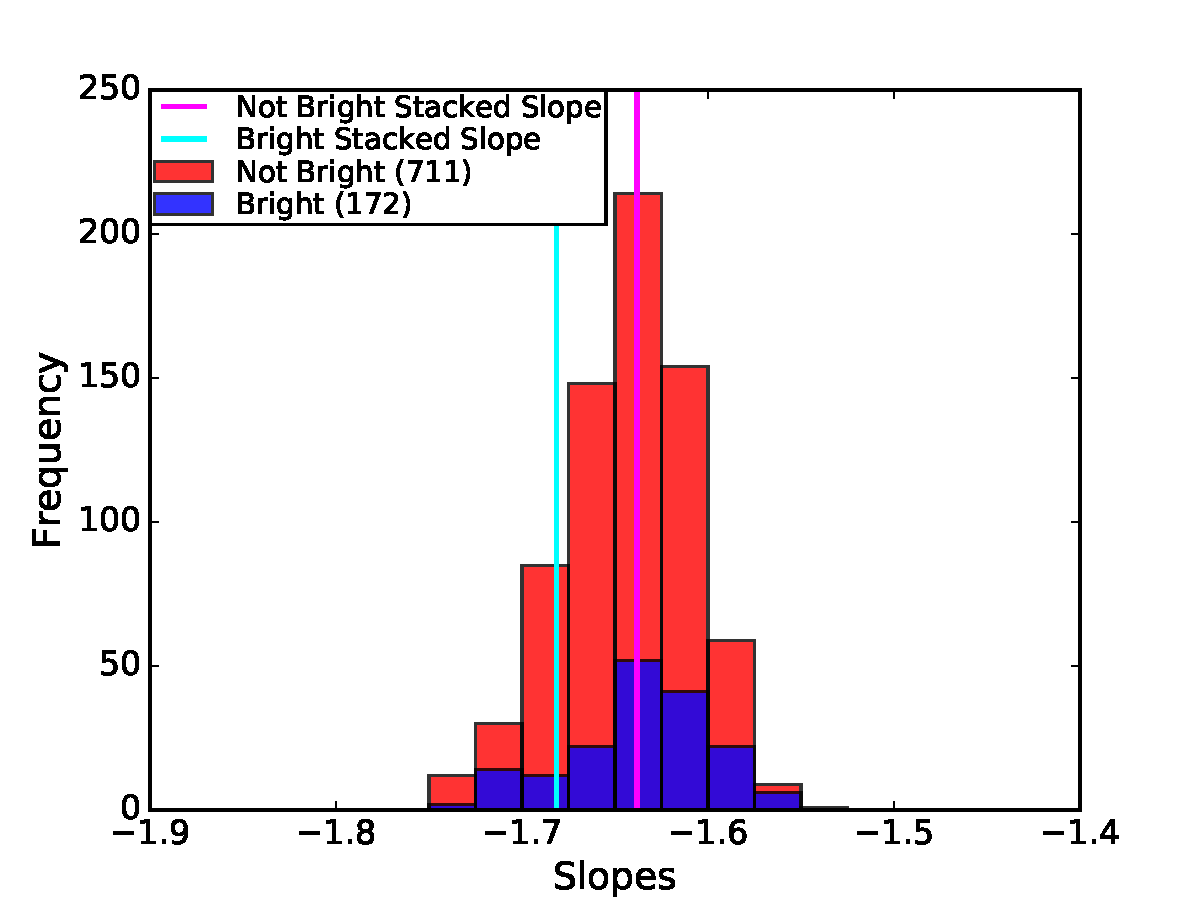
\includegraphics[width=0.5\textwidth]{3meanuplimslopedist.pdf}}
 \caption{With redshift cut: Stacked Luminosity Profile for LRG's flagged as Bright Center Objects (blue points), and those not flagged as Bright Center Objects (red points). }
\label{fig:mesh1}
\end{figure}

Figure \ref{fig:mesh1} shows stacked luminosity profile for each flagged (blue points) and non-flagged populations (red points). In the background, I plot the luminosity profiles of the individual galaxies (gray curves).  In order to homogenize our results, so they are all fit to the same physical boundary, we set an outer boundary of exactly 6r1/2 to both individual luminosity profiles and stacked profiles. As seen in Figure \ref{subfig:sfiga}, by removing the largest apertures from the profile, the mean slope of the galaxies flagged as bright center objects is now consistent (within the scatter) with that of the non-flagged galaxies. This indicates we have removed any parts of the profile at risk of contamination from un-blended sources at the bright galaxies� envelope, which caused the shallower slopes. By implementing this outer limit, we can safely use photometry of these bright sources.

Interestingly, we see that galaxies flagged as bright objects are in agreement with those not flagged. While there appears to be no real difference, we next need to check how these flags alter specific tests we want to accomplish.

\section{SFH and Bright Center Objects}
One test this project is performing is the relationship between the luminosity profile slopes and star formation history (SFH). We use the VESPA code, which fits the spectra of all LRGs in the Sloan Digital Sky Survey's (SDSS) final data release. After matching this catalogue with the LOWZ galaxies, we next separate the LRGs into two different populations, based on whether or not 60\% of the mass of the galaxy is formed in the oldest age bin (between 9.06 and 14 billion years ago). It is important to note that these are all early type galaxies, but we are still distinguishing them by SFH.

\begin{figure*}[h!]
\subfloat[Luminosity Density Profiles\label{subfig:sfig1}]{ 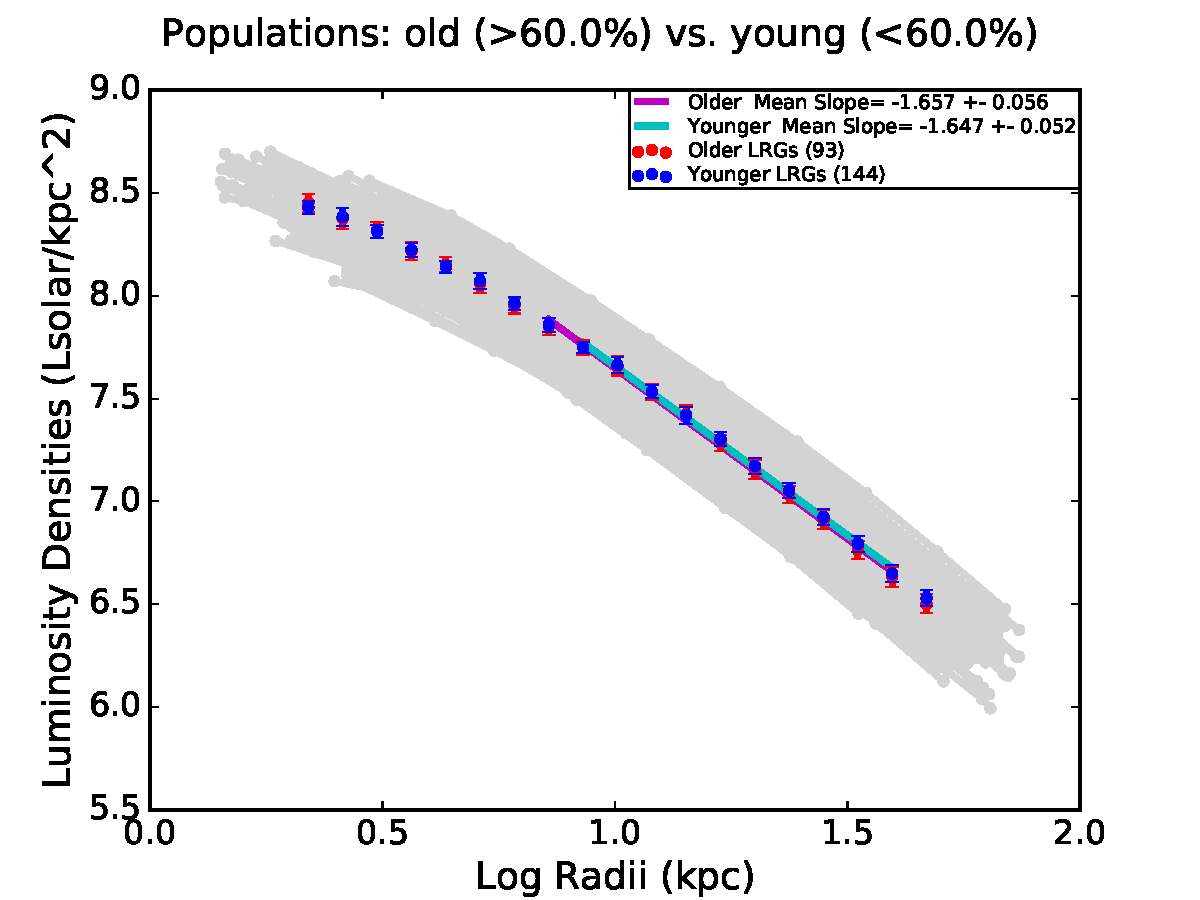
\includegraphics[width=0.5\textwidth]{3oymeanuplimlumage.pdf}}
\hfill
\subfloat[Distribution of alpha\_star slopes\label{subfig:sfig2}]{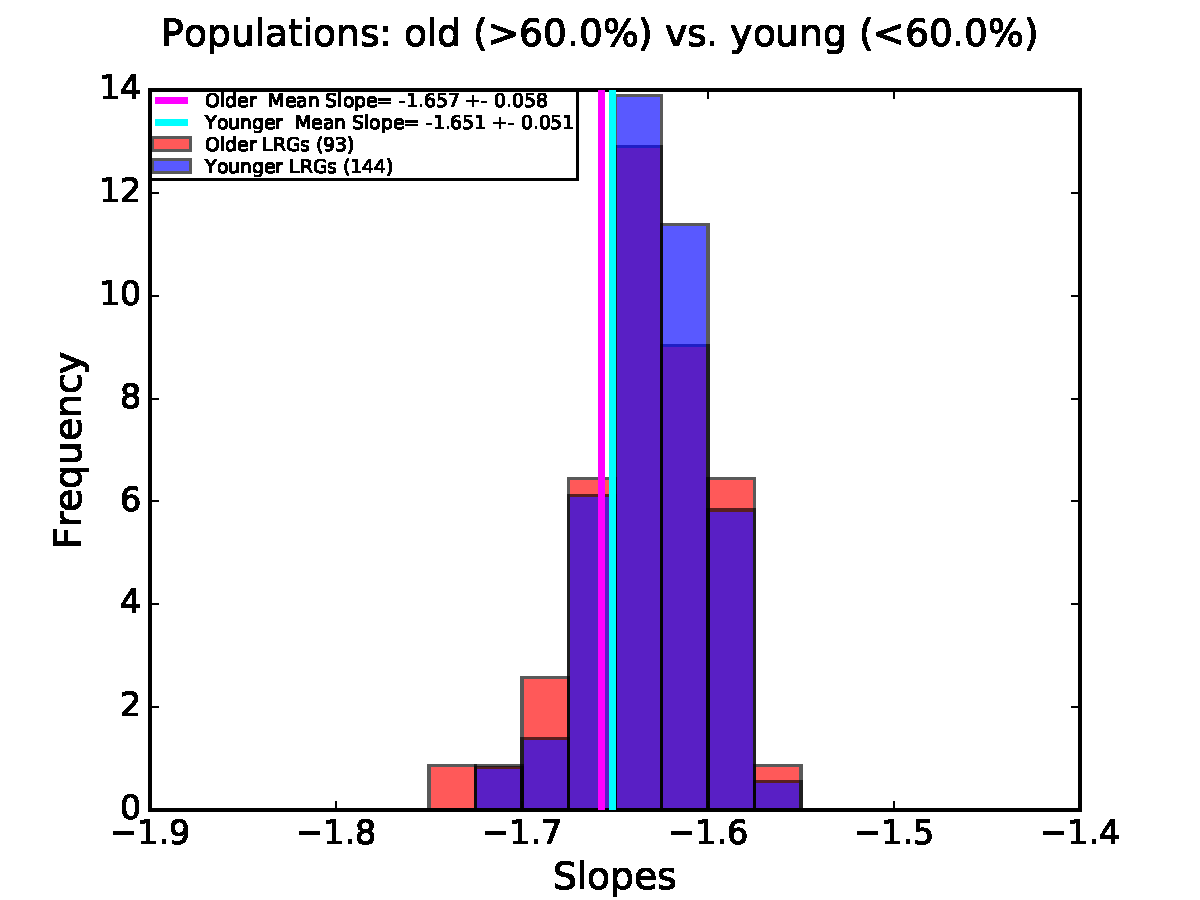
\includegraphics[width=0.5\textwidth]{3oymeanuplimslope_agedist.pdf}}
 \caption{In \ref{subfig:sfig1}, the luminosity profiles of older galaxies (red points) and younger galaxies (blue points). \ref{subfig:sfig2} reveals the distribution of alpha\_star slopes for both populations, as well as the stacked slopes (vertical lines).}
\label{fig:mesh2}
\end{figure*}


In Figure \ref{subfig:sfig1}  the stacked slopes of older and younger populations of LRGs appear to be roughly the same. Figure \ref{subfig:sfig2}reveals that their slope distributions, as well, are very similar.  The stacked slopes coincide with the gaussian distribution within one $\sigma$. However, in order to completely understand our results, we must see how bright center objects affect the luminosity profiles of both the older and younger galaxies.

\begin{figure*}[h!]
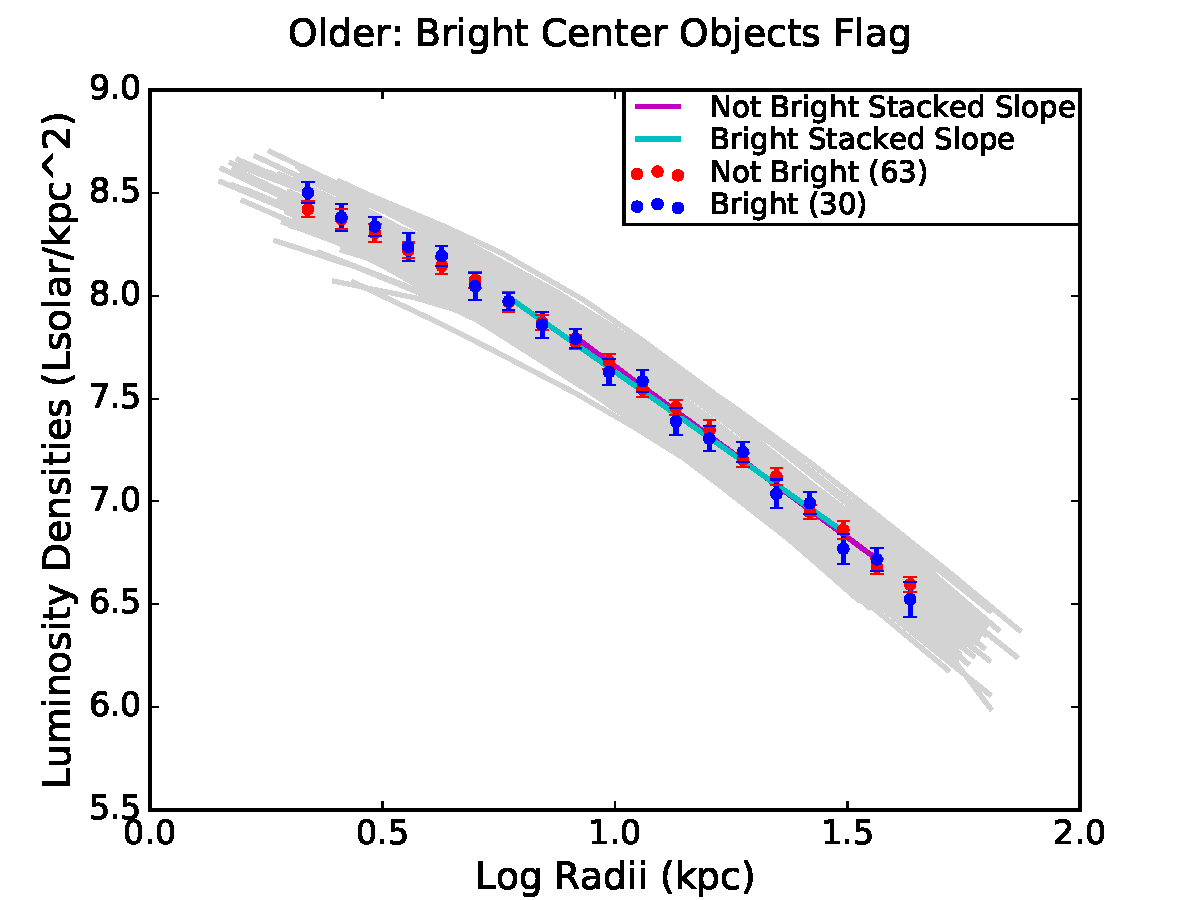
\includegraphics[width=0.5\textwidth,clip]{3oFmeanuplimlumage.pdf}
\label{subfig:sfig3}
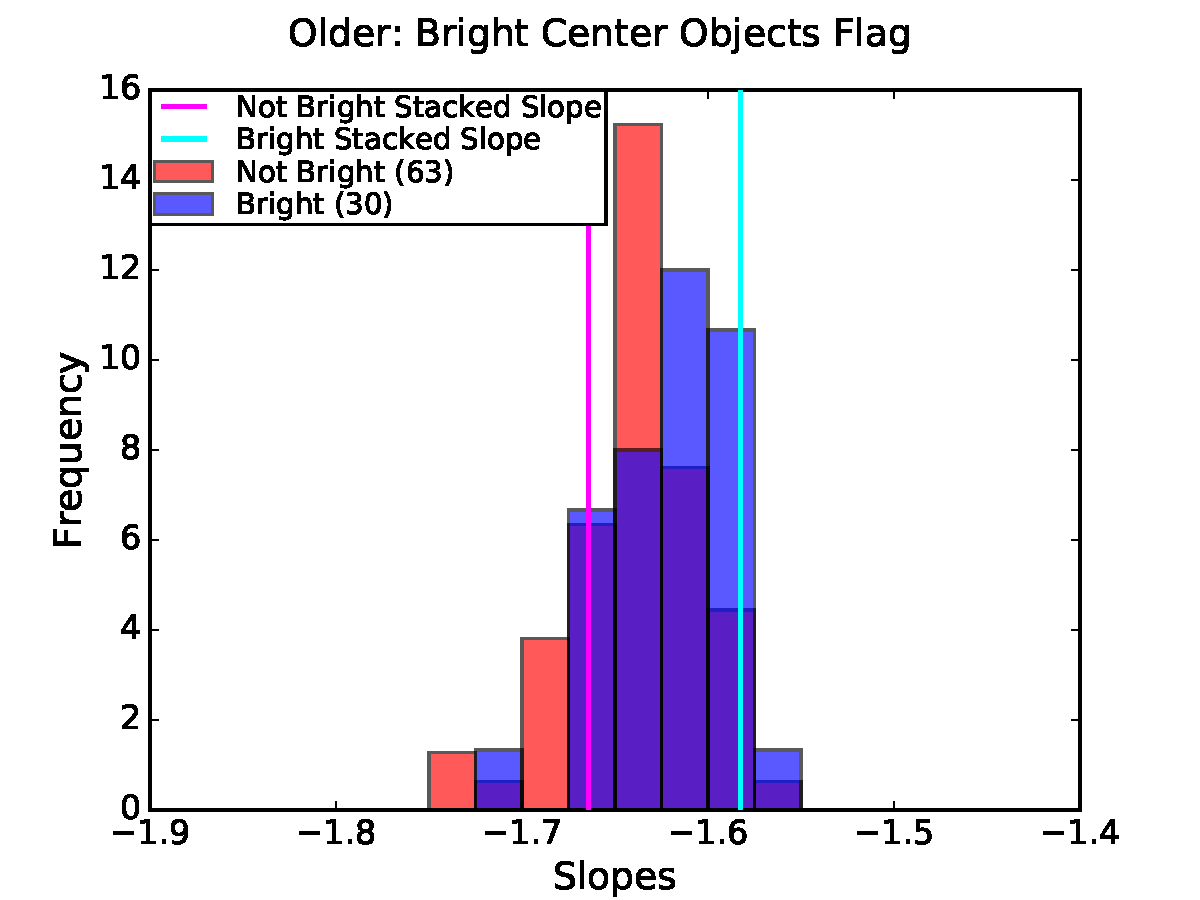
\includegraphics[width=0.5\textwidth,clip]{3oFmeanuplimslope_agedist.pdf}
\label{subfig:sfig4}
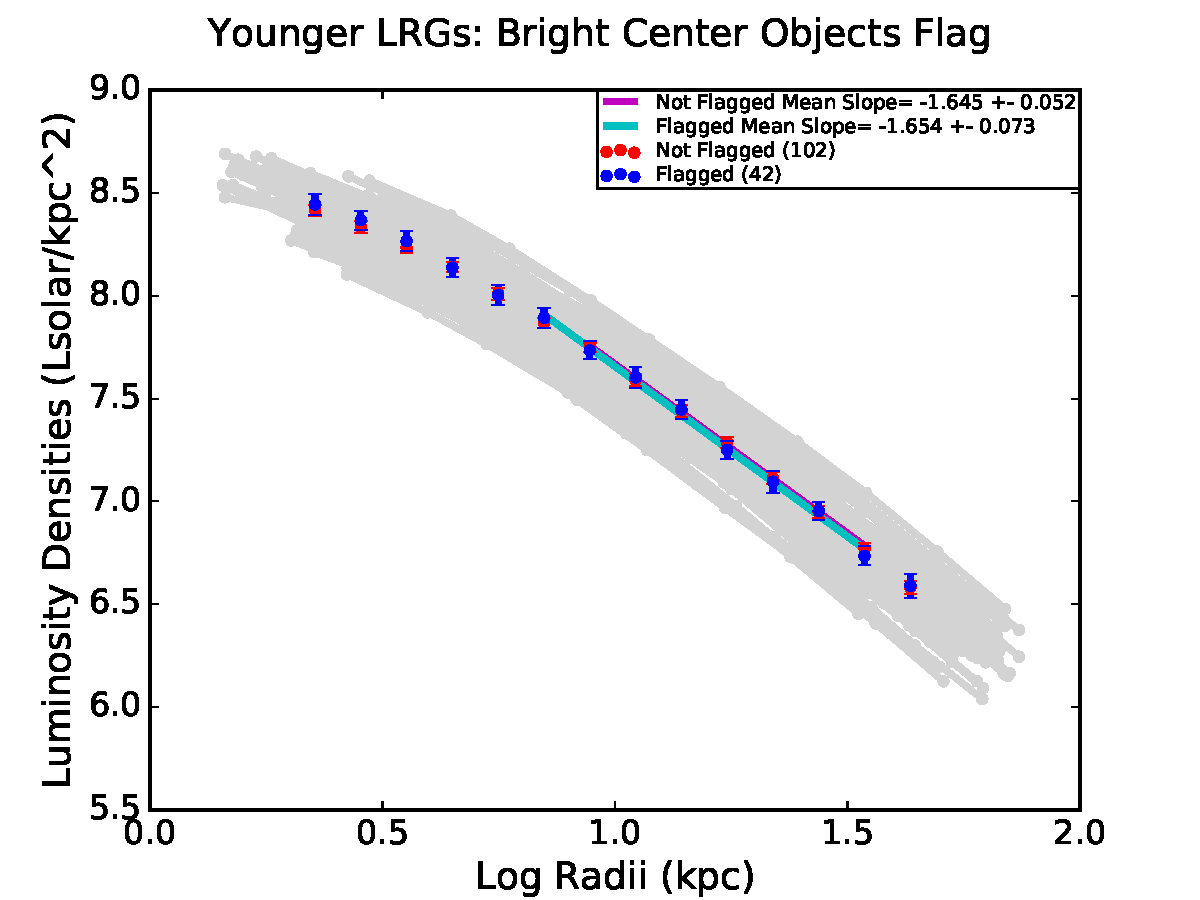
\includegraphics[width=0.5\textwidth,clip]{3yFmeanuplimlumage.pdf}
\label{subfig:sfig5}
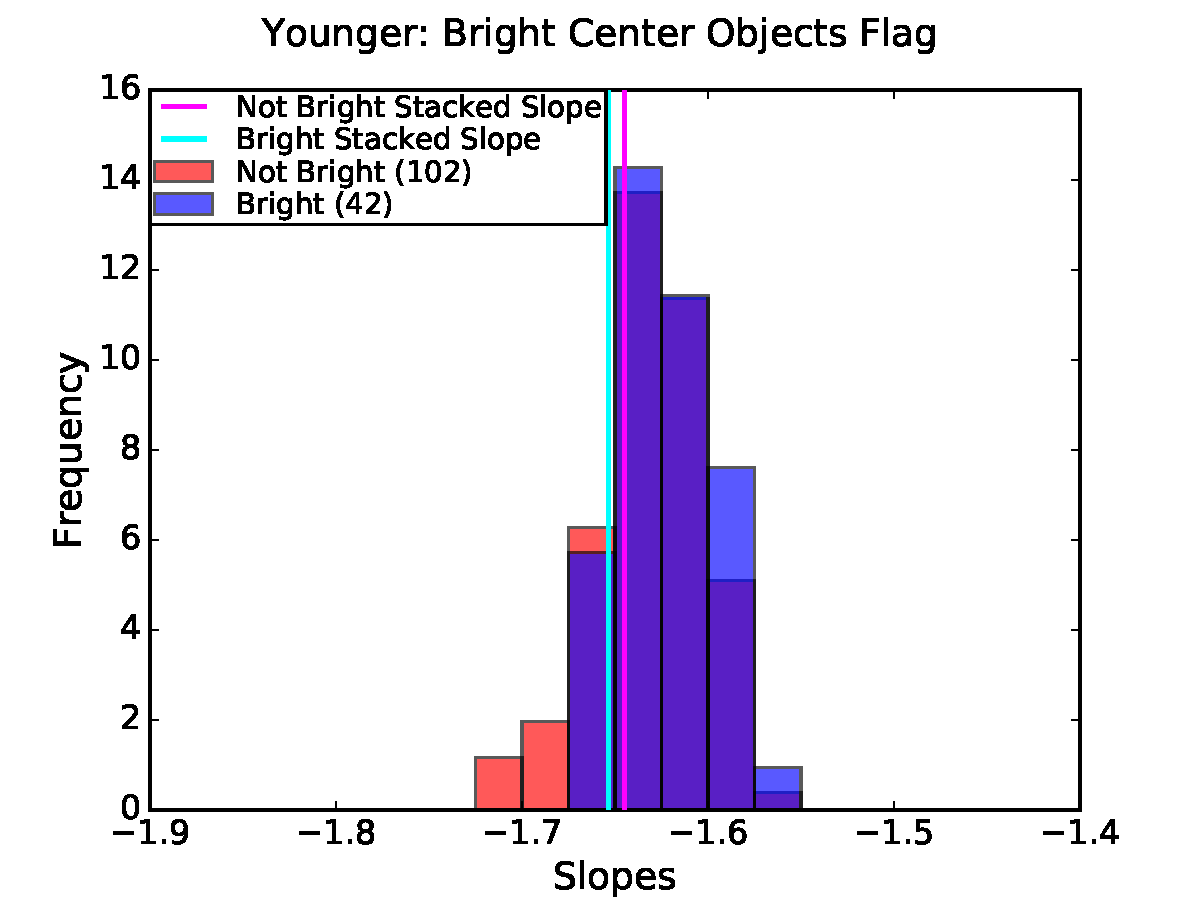
\includegraphics[width=0.5\textwidth,clip]{3yFmeanuplimslope_agedist.pdf}
\label{subfig:sfig6}
\caption{The left\-hand column shows the luminosity profiles of older (upper) and younger (lower) galaxies. Flagged Bright Object Centers are blue points and Not Flagged are red points. The right\-hand column shows the alpha\_star distribution amongst galaxies for flagged (blue bars) and not flagged (red bars). The stacked slopes are represented by the magenta and cyan vertical lines.}
\label{fig:mesh3}
\end{figure*}

In Figure \ref{fig:mesh3}, I separately show the older and younger populations of galaxies, further splitting into flagged (blue points) and not flagged(red points). In the right\-hand column, the stacked slopes of is in agreement with the distribution of individual slopes. This is validated in Table \ref{table:2}, which compares the alpha\_star slopes of the stacked galaxies with the median of the slope distribution for each subsample. Here, we see that, within error, the stacked slopes of the subsamples for older and younger galaxies agree with the stacked slopes of the larger older and younger populations.

In accordance with Figure \ref{subfig:sfigb}, there is no significant difference between the flagged and not flagged stacked luminosity profiles for both the older and younger galaxies as seen in the right hand side of Figure \ref{fig:mesh3}. 

\begin{table}[h!]
\centering
\begin{tabular}{ ||c|c|c|| }
\hline
\multicolumn{3}{||c||}{Distribution of Alpha\_Star Slopes}\\
\hline\hline
   & Stacked Slope & Median Slope \\
\hline
All Not Flagged & -1.64  $\pm$  0.02 & -1.64\\
\hline
All Flagged & -1.68  $\pm$  0.06 &-1.63\\
\hline
Old Galaxies & -1.66  $\pm$  0.06 & -1.63 \\
\hline
Young Galaxies & -1.65  $\pm$  0.05 & -1.629\\
\hline
Old and Not Flagged & -1.66  $\pm$  0.05&  -1.633\\
\hline
Old and Flagged & -1.58  $\pm$  0.07 &  -1.619\\
\hline
Young and Not Flagged &-1.64  $\pm$  0.05 & -1.629\\
\hline
Young and Flagged & -1.65  $\pm$  0.07 & -1.623\\
\hline
\end{tabular}
\caption{These stacked and median slopes were calculated from specific population's individual galaxy slope distribution}
\label{table:2}
\end{table}



\end{document}